%
% intfun.tex -- Beispiel integrierbarerer aber nicht quadratintegrierbare Fkt.
%
% (c) 2019 Prof Dr Andreas Müller, Hochschule Rapperswil
%
\documentclass[tikz]{standalone}
\usepackage{amsmath}
\usepackage{times}
\usepackage{txfonts}
\usepackage{pgfplots}
\usepackage{csvsimple}
\usetikzlibrary{arrows,intersections,math}
\begin{document}
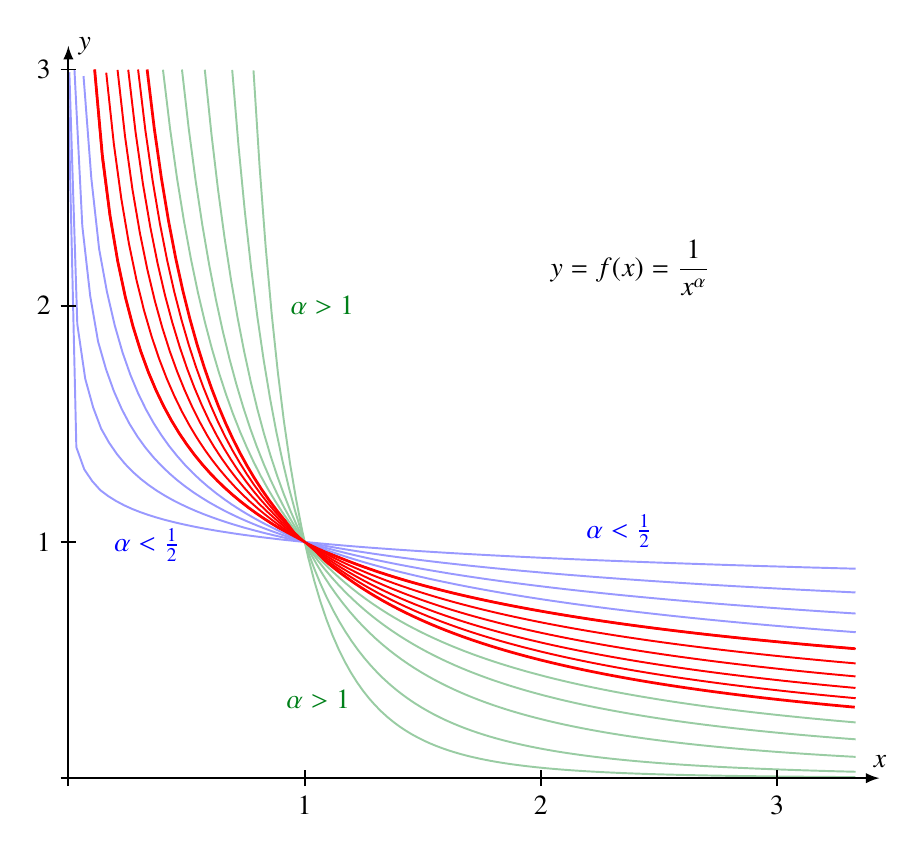
\begin{tikzpicture}[>=latex]

\draw[color=red,line width=1pt] plot[domain={1/3}:3.33,samples=100]
	({3*\x},{3/\x});
\draw[color=red,line width=1pt] plot[domain={1/9}:3.33,samples=100]
	({3*\x},{3/sqrt(\x)});

\foreach \a in {0.1,0.2,0.3,0.4}{
	\draw[color=blue!40,line width=0.7pt]
		plot[domain={exp(-ln(3.0)/\a)}:3.33333,samples=100]
			({3*\x},{3/exp(\a*ln(\x))});
}

\definecolor{darkgreen}{rgb}{0,0.5,0.1}

\foreach \a in {1.2,1.5,2,3,4.5}{
	\draw[color=darkgreen!40,line width=0.7pt]
		plot[domain={exp(-ln(3.0)/\a)}:3.33333,samples=100]
			({3*\x},{3/exp(\a*ln(\x))});
}

\foreach \a in {0.5,0.6,...,1}{
	\draw[color=red,line width=0.7pt]
		plot[domain={exp(-ln(3.0)/\a)}:3.33333,samples=100]
			({3*\x},{3/exp(\a*ln(\x))});
}

\draw[->,line width=0.7pt] (0,-0.1)--(0,9.3) coordinate[label={right:$y$}];
\draw[->,line width=0.7pt] (-0.1,0)--(10.3,0) coordinate[label=$x$];

\draw[line width=0.7pt] (3,-0.1)--(3,0.1);
\draw[line width=0.7pt] (6,-0.1)--(6,0.1);
\draw[line width=0.7pt] (9,-0.1)--(9,0.1);
\node at (3,-0.1) [below] {$1$};
\node at (6,-0.1) [below] {$2$};
\node at (9,-0.1) [below] {$3$};

\draw[line width=0.7pt] (-0.1,3)--(0.1,3);
\draw[line width=0.7pt] (-0.1,6)--(0.1,6);
\draw[line width=0.7pt] (-0.1,9)--(0.1,9);
\node at (-0.1,3) [left] {$1$};
\node at (-0.1,6) [left] {$2$};
\node at (-0.1,9) [left] {$3$};

\node[color=blue] at (7,2.8) [above] {$\alpha < \frac12$};
\node[color=blue] at (1,3.3) [below] {$\alpha < \frac12$};

\node[color=darkgreen] at (2.7,6) [right] {$\alpha > 1$};
\node[color=darkgreen] at (3.7,1) [left] {$\alpha > 1$};

\node at (6,6) [above right] {$\displaystyle y=f(x)=\frac{1}{x^\alpha}$};

\end{tikzpicture}
\end{document}

